\chapter{Charakterystyka EPUB}

EPUB jest standardem formatu dystrybucji cyfrowych publikacji i dokumentów opartych na standardach technologii webowej. EPUB definiuje formę reprezentacji, organizacji struktury oraz kodowania określonej zawartości webowej, na co składają się XHTML, CSS, SVG, obrazy i inne zasoby sprowadzone do formy pojedynczego pliku. EPUB daje wydawcom możliwość stworzenia cyfrowej publikacji, a następnie dystrybuowania go, a odbiorcy łatwy dostęp do pliku niezależnie od urządzenia jakim operuje. Jako następca OEB (Open eBook Publication Structure, zaprezentowanego w 1999 roku, EPUB 2 został ustandaryzowany w roku 2007, a aktualną jego wersją jest EPUB 3.1 (styczeń 2017). Dzisiaj jest on standardem wykorzystywanym na szeroką skalę przez wszystkich wydawców. Obok MOBI oraz PDF dominuje na rynku, dzięki jego popularności wśród wydawców oraz wsparciu urządzeń. W przeciwieństwie do MOBI, które zostało spopularyzowane przez Amazon, właściciela sklepu amazon.com, giganta dystrybucji książek elektronicznych oraz producenta czytników elektronicznych marki Kindle, EPUB jest standardem uniwersalnym, nieograniczonym do jednej platformy. EPUB zarówna jak i MOBI charakteryzuje się tym, że jego zawartość nie jest statyczna, co oznacza, że ilość która jest wyświetlana dopasowana jest do wielkości ekranu urządzenia, dzięki czemu jest ona bardziej przyjazna dla odbiorcy. PDF natomiast jest już podzielony na strony których nie da się podzielić. To co najbardziej różni EPUB od MOBI, to wsparcie EPUB dla multimediów (od wersji 3.0) oraz CSS, który stylizuje cały dokument. Dzięki temu jest znacznie bardziej elastyczny i nowoczesny. Popularną praktyką wśród dystrybutorów książek elektronicznych, jest dostarczanie książki klientowi, który ją zakupił we wszystkich trzech wcześniej wymienionych formatach. EPUB jako standard jest szeroko udokumentowany dzięki International Digital Publishing Forum\footnote{Adres url: \href{idpf.org}{idpf.org}}, grupie która nadzoruje rozwój formatu. W następnej sekcji zostanie szczegółowo opisana struktura formatu EPUB.

\section{Specyfikacja}

Poniższa specyfikacja jest podzbiorem najważniejszych informacji wyselekcjonowanych ze specyfikacji EPUB 3.1 z dnia 5-go stycznia 2017 roku, dostępnej na stronie International Digital Publishing Forum \footnote{Adres url najnowszej wersji specyfikacji: \href{http://www.idpf.org/epub3/latest}{http://www.idpf.org/epub3/latest}}. Przedstawiono tutaj najbardziej istotne elementy formatu EPUB w celu zrozumienia problemu jakiego dotyczy projekt EPUBKit.

\subsection{EPUB Open Container Format}

\begin{figure}[ht!]
  \centering
  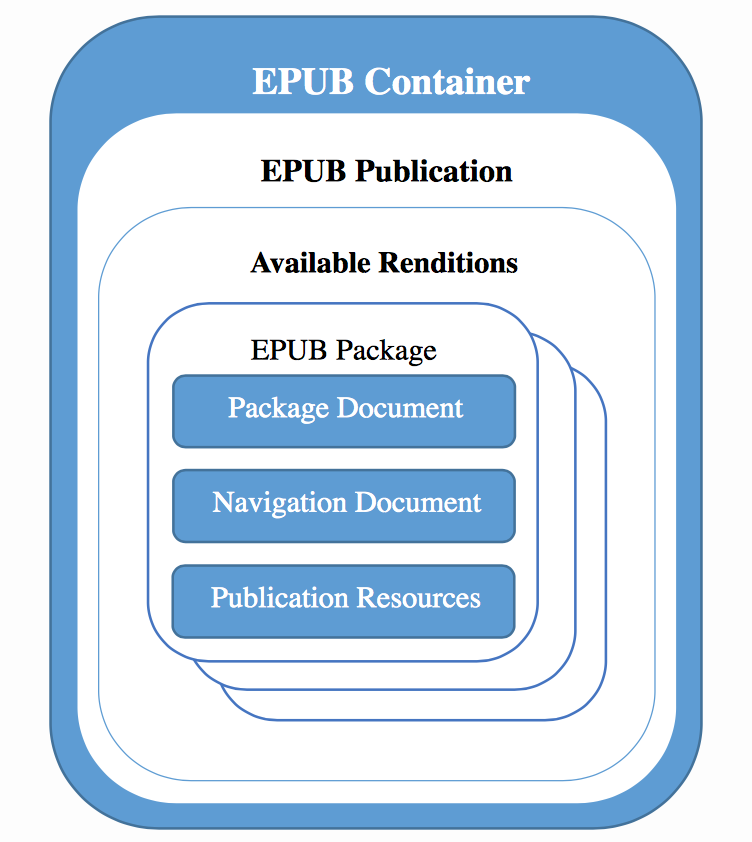
\includegraphics[width=.4\linewidth]{images/chapter-3-image-1-structure.png}
  \caption{Wizualna reprezentacja struktury formatu EPUB\cite{EPUBSpecification}}
  \label{fig:epubspec}
\end{figure}

Format EPUB definiuje jego najwyższy abstrakcyjny model jakim jest EPUB Publication(patrz: rysunek \ref{fig:epubspec}). Model ten składa się z interpretacji jego zawartości. Interpretacja, która jest przedstawiona za pomocą EPUB Package, zawiera już bezpośrednio zawartość dokumentu, oraz poboczne zasoby mające na celu wspomagać system czytający (z ang. ze specyfikacji \textit{Reading System}, jakim jest EPUBKit). Kluczowym elementem jest Package Document, który zawiera wszystkie metadane, które są używane następnie przez system czytające do zaprezentowania publikacji użytkownikowi. Zawiera on również kompletny manifest zasobów publikacji oraz \textit{kręgosłup} (z ang. ze specyfikacji \textit{Spine}), który reprezentuje sekwencję w jakiej system czytający ma wyświetlać poszczególne elementy. EPUB Package zawiera również Navigation Document pełniący rolę spisu treści, przeznaczony dla użytkownika do poruszania się po dokumencie. Wszystko to opakowane jest w archiwum ZIP z rozszerzeniem .epub. Rozszerzenie informuje o charakterze pliku oraz dostarcza informację o archiwum w ZIPowskim stylu za pomocą pliku \textit{mimetype}, oraz zapewnia system o posiadaniu przez niego folderu \texttt{/META-INF}, w którym dostępny jest plik \texttt{container.xml}, niezbędny systemowi do określenia lokalizacji zawartości publikacji.

\begin{lstlisting}[caption={Przykładowy plik container.xml}, language=XML,label=container-xml]
<?xml version="1.0" encoding="UTF-8"?>
<container version="1.0" xmlns="urn:oasis:names:tc:opendocument:xmlns:container">
    <rootfiles>
        <rootfile full-path="OEBPS/content.opf" media-type="application/oebps-package+xml"/>
   </rootfiles>
</container
\end{lstlisting}

To w jaki sposób zawartość publikacji jest zorganizowana, określa standard EPUB Open Container Format (OPF), który definiuje reguły enkapsulacji zasobów w pojedynczym kontenerze abstrakcyjnym (EPUB Container) zawartym w archiwum ZIP. Struktura OPF to tylko jedna część składająca się na EPUB Publication, druga część to zawartość przedstawiona użytkownikowi, która jest oparta o dokumenty określone w specyfikacji jako EPUB Content Documents. Zawartość ta jest rozszerzona o wiele dodatkowych zasobów potrzebnych do prawidłowego wyświetlenia publikacji jakimi mogą być obrazy, pliki audio lub video, dodatkowe czcionki, skrypty oraz style nazywane w oficjalnej specyfikacji \textit{EPUB Core Media Types}.

\subsection{EPUB Content Documents}

Ta sekcja opisuje rolę jaką odgrywają standardy HTML, SVG i CSS w elektronicznej publikacji w formacie EPUB. Wizualna kompozycja publikacji w znacznej mierze oparta jest o pliki XHTML. Specyfikacja EPUB Content Documents 3.1 szczegółowo opisuje semantykę atrybutów wspieranych przez EPUB, które mają na celu wzbogacenie doświadczenia użytkownika. Tak jak pokazano na przykładzie \ref{epub-sample-attribute} atrybuty te nadają dodatkową naturę i znaczenie elementom XHTML, przy tym nie nadpisując ich pierwotnej funkcjonalności. Atrybuty te są przeznaczone wyłącznie dla systemów czytających i przekazują istotne informacje odnośnie struktury i zawartości dokumentu. Wsparcie standardu EPUB dla HTML nie odnosi się do konkretnej jego wersji, natomiast pozostawia tę kwestię twórcom systemów czytających. To w ich obowiązkach leży upewnienie się, że każda publikacja zostanie prawidłowo przez system obsłużona.

\begin{lstlisting}[float=h, caption={Przykładowe wykorzystanie atrybutu epub:type aby oznaczyć zakończenie linii.\protect\cite{EPUBContentDocumentsSpecification}}, language=XML, label=epub-sample-attribute]
<html ... xmlns:epub="http://www.idpf.org/2007/ops">
   ...
   <p> ... <span epub:type="pagebreak" title="234" id="p234"/> ... </p>
   ...
</html>
\end{lstlisting}

Kolejnym typem dokumentu ważnym dla formatu EPUB jest SVG (Scalable Vector Graphics). Co prawda uniwersalność XHTML przyczynia się do tego iż jest to w znacznej mierze dominujący format przedstawiania treści w publikacji, SVG oferuje udogodnienia dzięki czemu również znajduje zastosowanie. Format ten jest zazwyczaj wykorzystywany w specyficznych przypadkach, takich jak prezentacja zawartości publikacji z gatunku manga czy komiks. Użytkownik oczekiwał by od tego typu dokumentu, aby zawartość w tym przypadku głównie graficzna, prezentowała się dobrze na każdym urządzeniu niezależnie od rozdzielczości jego ekranu, i to właśnie SVG może zagwarantować. Dodatkowo, treść tych dokumentów jest zazwyczaj z góry podzielona na strony, i narzuca systemom czytającym wyświetlenie ich w określonej formie.

CSS odgrywa ogromną rolę w praktyce programistycznej jako technologii webowej od wielu lat, i jego możliwości wciąż rosną. Nietrudno się domyślić, że swoje miejsce CSS znajduje również w standardzie EPUB. Prezentacja publikacji jest sztywnie ustylizowana, chociaż nadpisywanie stylu przez systemy czytające nie jest zabronione. Specyfikacja EPUB sugeruje, aby systemy dawały możliwość zmian w stylu publikacji użytkownikowi, który dopasuje jej wygląd pod swoje upodobania. Zazwyczaj będzie to kolor tła, rozmiar czy typ czcionki. Specyfikacja również przestrzega twórców publikacji w formacie EPUB, aby rozważnie stylizować dokument. Niektóre systemy czytające mogą nie wspierać pewnych elementów CSS co może być problematyczne \cite{EPUBContentDocumentsSpecification}.

To o czym również należy wspomnieć opisując EPUB Content Documents jest to, że EPUB wspiera skrypty w dokumentach HTML czy SVG. Opcjonalne jest wspieranie skryptowania w systemach czytających, natomiast te systemy, które wspierają skryptowane dokumenty, muszą wziąć pod uwagę pewne niebezpieczeństwa z tym związane. Specyfikacja przestrzega, aby systemy czytające zapewniały izolację publikacji w celu uniknięcia niebezpieczeństw zagrażającym podatnej na ataki zawartości. System powinien monitorować wszelkie aktywności, aby zawartość pozostała nienaruszona. Należy założyć, że może zostać przeprowadzony atak na zawartość innych plików w strukturze publikacji, atak na sam system czytający, np. próba zdobycia danych użytkownika, lub atak na sieć czy wszczepianie innych złośliwych skryptów w niezaszyfrowane fragmenty dokumentu. Ponadto systemy które zezwalają na stałe przechowywanie publikacji muszą dostarczyć metody zezwalające na podgląd i kasowanie danych publikacji. W sytuacji usunięcia publikacji przez użytkownika, system musi skasować wszelakie pliki z nią związane \cite{EPUBContentDocumentsSpecification}.

\subsection{EPUB Core Media Types}

Zaobserwować można, że EPUB jako format jest bardzo ściśle wyspecyfikowany odnośnie jego struktury i wspieranych technologii. W przypadku samej zawartości nie jest inaczej. Specyfikacja EPUB 3 Core Media Types\footnote{Adres url: \href{https://idpf.github.io/epub-cmt/v3/}{https://idpf.github.io/epub-cmt/v3/}} szczegółowo opisuje jakie typy mediów mogą zostać załączone do publikacji i określa dla nich unikalny typ (\textit{Media Type}), który jest wykorzystywany w celach poinformowania systemu czytającego o typie danego elementu. Ta sekcja opisuje poszczególne typy mediów wspierane przez EPUB, nie zagłębiając się przy tym w techniczne szczegóły konkretnego typu.

\subsubsection*{Image Types}

Wspierane typy obrazów (\textit{Image Types}) to GIF, JPEG, PNG oraz SVG. Ich typy zadeklarowane w standardzie EPUB to kolejno \textit{image/gif}, \textit{image/jpeg}, \textit{image/png}, \textit{image/svg+xml}. Notacja ta wykorzystywana jest w atrybutach elementów wskazujących na konkretny obiekt odpowiedniego typu. Oznaczenia te możemy spotkać w manifeście publikacji.

\begin{lstlisting}[caption={Przykładowy fragment manifestu znajdującego się w pliku content.opf}, language=XML,label=sample-manifest]
<manifest>
  ...
  <item href="Images/image-1.jpg" id="id1" media-type="image/jpeg"/>
  <item href="Images/image-2.jpg" id="id2" media-type="image/jpeg"/>
  ...
</manifest>
\end{lstlisting}

Sposób oznaczenia elementów zademonstrowany na przykładzie \ref{sample-manifest}, wykorzystywany jest w deklarowaniu każdego obiektu o wspierany przez EPUB typie.

\subsubsection*{Audio Types}

EPUB wspiera pliki audio w formacie MP3 (\textit{audio/mpeg}) oraz MP4 (\textit{audio/mp4}). Zapewne zdecydowano się na te dwa konkretne standardy ze względy na ich popularność oraz mały rozmiar dzięki stosunkowo wysokiej kompresji.

\subsubsection*{Video Types}

Ze względu na rozbieżność preferencji wśród autorów oraz twórców specyfikacji, EPUB nie definiuje preferowanego typu wideo dla publikacji w swoim standardzie. IDPF proponuje dwa formaty kodowania: H.264 oraz WebM, ale nie kładzie nacisku na jeden z nich. Tę kwestię pozostawia na ten moment autorom. Spór dotyczący określenia konkretnego formatu plików wideo rozchodzi się o szerokie wsparcie H.264 przeciwko nieopatentowanemu, wolnemu formatowi WebM, który jednak wciąż nie jest spopularyzowanym standardem. IDPF deklaruje, że najprawdopodobniej w pewnym momencie preferowany standard zostanie określony, jednakże teraz jest jeszcze na to zbyt wcześnie \cite{WhatIsEPUB3Video}.

\subsubsection*{Application, Text, Font Types}

Pozostałe typy które wspiera EPUB zdecydowano się opisać razem w tej sekcji w skrócie ze względu na to, że wszystkie służą jednemu celowi jakim jest prezentacja treści. Są to czcionki w formacie WOFF(\textit{application/font-woff}), WOFF2(\textit{font/woff2}) oraz OpenType/TrueType(\textit{application/font-sfnt}), pliki CSS(\textit{text/css}), skrypty(\textit{application/javascript}), dokumenty XHTML(\textit{application/xhtml+xml}), nawigacyjne pliki NCX(\textit{application/x-dtbncx+xml}) oraz nakładki MediaOverlays3(\textit{application/smil+xml}) wraz z plikami PLS(\textit{application/pls+xml}), które mają na celu odtworzenia tekstu w formie dźwiękowej\cite{EPUBCoreMediaTypes}.

\subsubsection*{Foreign Resources}

Należy wspomnieć, iż EPUB zezwala na użycie niewspieranych formatów, jednakże nie gwarantuje, że zostaną prawidłowo obsłużone przez systemy czytające, od których wymaga jedynie wsparcia wcześniej wymienionych formatów. W przypadku użycia przez autora publikacji niewspieranych formatów, specyfikacja EPUB wymaga od niego zadeklarowanie tak zwanego \textit{Core Media Type fallback}, czyli typu wspieranego, który zastępczo będzie przypisany do obiektu jeżeli system czytający nie będzie wspierał pierwotnie wskazanego typu \cite{EPUBSpecification}.
